\documentclass[a4paper]{scrreprt}

%% Language and font encodings
\usepackage[brazil]{babel}
\usepackage[utf8]{inputenc}
\usepackage[T1]{fontenc}
\usepackage{float}

%% Sets page size and margins
\usepackage[a4paper,top=3cm,bottom=2cm,left=3cm,right=3cm,marginparwidth=1.75cm]{geometry}

%% Useful packages
\usepackage{amsmath}
\usepackage{graphicx}
\usepackage[colorinlistoftodos]{todonotes}
\usepackage[colorlinks=true, allcolors=blue]{hyperref}
\usepackage{listings}
\usepackage{xcolor}

\lstset{
    language=Python,           % Linguagem do código
    basicstyle=\ttfamily,      % Fonte monoespaçada
    keywordstyle=\color{blue}, % Cor para palavras-chave
    commentstyle=\color{gray}, % Cor para comentários
    stringstyle=\color{red},   % Cor para strings
    numbers=left,              % Numeração das linhas
    numberstyle=\tiny\color{gray}, % Estilo dos números
    stepnumber=1,              % Numera todas as linhas
    frame=single,              % Moldura ao redor do código
    tabsize=4,                 % Tamanho do tab
    breaklines=true,           % Quebra linhas longas
    breakatwhitespace=false,   % Não quebra apenas em espaços
    showstringspaces=false,    % Não mostra espaços em strings
}

\title{Tombshifter}
\subtitle{Roguelike minimalista ambientado em tumbas}
\author{Gabriel Sales, Romulo Goes}



\begin{document}
\maketitle

\newpage

\begin{abstract}
Tombshifter se trata de um jogo para computador do tipo "Roguelike", com inspirações em The Legend of Zelda: A Link to the Past e The Binding of Isaac: Rebirth, Tombshifter traz uma proposta de jogo minimalista contendo as principais características de um jogo do gênero. Tal jogo foi desenvolvido por meio do framework PPlay desenvolvido na Universidade Federal Fluminense e será apresentado na disciplina de Laboratório de Desenvolvimento de Jogos, lecionada pelo Prof. Dr. Esteban Walter Gonzalez Clua, como método de avaliação. 
\end{abstract}

\tableofcontents

% ______________________
% chapter Overview
% ______________________
\chapter{Visão Geral}
    Tombshifter apresenta a proposta de um jogo desenvolvido principalmente com o intuito de compreender e aplicar os fundamentos de desenvolvimento de jogos. Isso foi feito por meio do desenvolvimento pelo framework PPlay, escrito na linguagem Python.

    Apresenta como principal característica a câmera "Top-Down", a qual se mostra bem presente em jogos do gênero. O jogo não apresenta mecânicas muito complexas pois o seu objetivo se limita a compreensão e pratica dos conceitos supracitados.

    Tem influência de jogos como The Legend of Zelda: A Link to the Past e The Binding of Isaac: Rebirth, similando-se pelos modos de ataque, movimentação e câmera, mas também se diferenciando pela proporção, proposta, estética e complexidade.


\section{Conceito Principal}
    O jogo se desenvolve de forma simples, pelos seguintes passos:
    \begin{itemize}
        \item Entrar em uma sala;
        \item Gerar inimigos;
        \item Derrotar os inimigos;
        \item Entrar em outra sala.
    \end{itemize}

    Com um limite de 10 de HP para o personagem principal, é gerado um grande desafio para o jogador que deseja completar o jogo que é composto por 10 fases.



% ______________________
% chapter References
% ______________________

\chapter{Referências} 
    Foram utilizados os seguintes jogos como referências:
    \begin{itemize}
        \item \textbf{The Binding of Isaac: Rebirth}
        
        Foram reaproveitadas a forma em que os inimigos são gerados e a forma de dar dano aos inimigos.
        
        \begin{figure}[H]
            \centering
            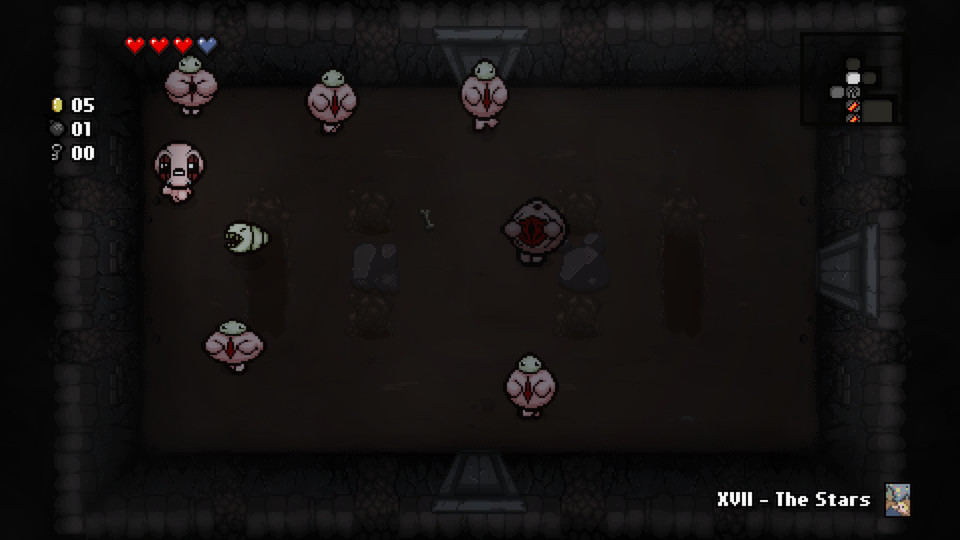
\includegraphics[width=.6\linewidth]{isac.jpg}
            \caption{Exemplo de The Binding of Isaac: Rebirth.}
            \label{fig:isac}
        \end{figure}
        
        \item \textbf{The Legend of Zelda: A Link to the Past}
        
        Foi reaproveitada grande parte da estética do jogo, incluindo alguns inimigos que são uma mistura de NPCs do mesmo.
        
        \begin{figure}[H]
            \centering
            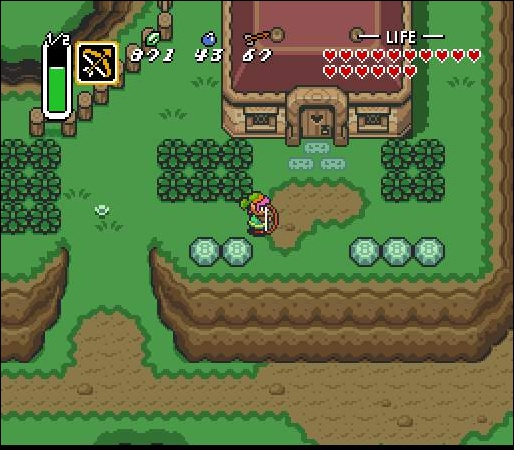
\includegraphics[width=.6\linewidth]{zelda.jpg}
            \caption{Exemplo de The Legend of Zelda: A Link to the Past.}
            \label{fig:zelda}
        \end{figure}
    \end{itemize}

% ______________________
% chapter Specification and Market Analysis 
% ______________________

\chapter{Especificações}

    \section{Público Alvo}
        O público alvo do jogo se dá principalmente para estudantes acadêmicos ou entusiastas da área de desenvolvimento de jogos para que possam ter um exemplo limpo de fundamentos de desenvolvimento de jogos. Mas também pode ser aproveitado como forma de entretenimento para qualquer interessado 

    \section{Gênero}
        Seu gênero é roguelike, que geralmente possui como característica uma gameplay simples, em 2D, com arenas fechadas e um desafio progressivo.

    \section{Estilo de Arte}
        O estilo de arte se dá pelo "Pixel-Art", muito presente em jogos desse escopo. Inimigos são releituras de outros inimigos do The Legend of Zelda citado na referência.


    \section{Formas de Diversão}
        Pensando nas 8 formas de diversão de Hunicke, Tombshifter se encaixa mais na comunhão, que se dá principalmente pela formação e participação em comunidades de desenvolvimento de jogos como o DJUFF (Desenvolvimento de Jogos da Universidade Federal Fluminense).

    % ______________________
    % chapter Game Details
    % ______________________


\chapter{Gameplay e Configurações} 

    \section{Humor e Emoções}
        A atmosfera do jogo trás uma leve sensação de desconforto ou ansiedade que é comum nesse tipo de jogo. A constante necessidade de desviar dos inimigos e ataca-los deixa o jogador em constante estado de alerta, principalmente pelo fato de que se o mesmo morrer, terá que começar do início.

    \section{História}
        Um ser é despertado e descobre que já não tem a mesma vitalidade de antes, pelo contrário, é um morto-vivo. O ser não se conforma com a situação e se vê na necessidade de escapar de sua tumba, para que assim possa tentar driblar o fim comum a todos nós.

    \section{Ambiente}
        O ambiente de jogo são 3 arenas de mesmo formato mas cores diferentes. Essas arenas são os andares da tumba em que o player se encontra.
            \begin{figure}[H]
                \centering
                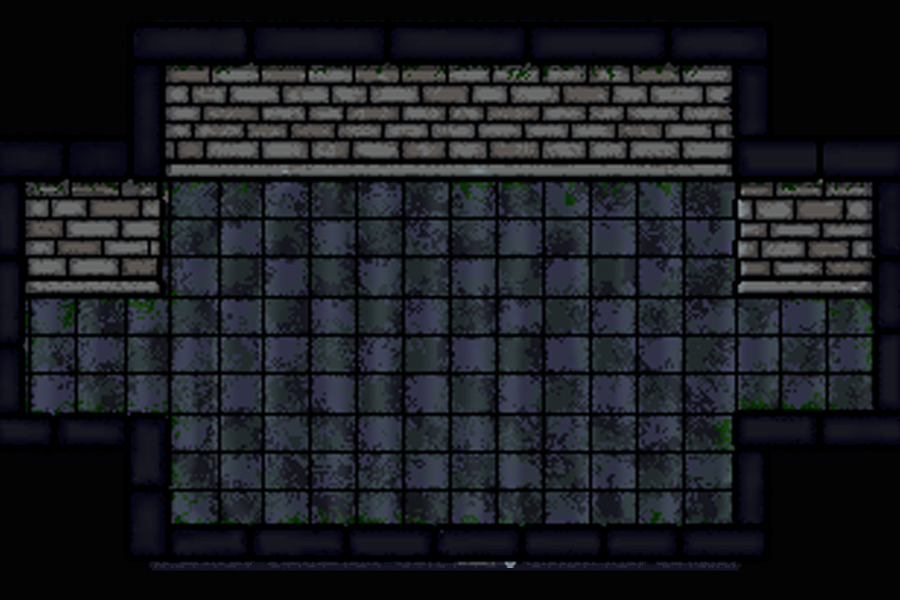
\includegraphics[width=.6\linewidth]{arena_2.png}
                \caption{Primeira arena do jogo}
                \label{fig:arena_2}
            \end{figure}
            
            \begin{figure}[H]
                \centering
                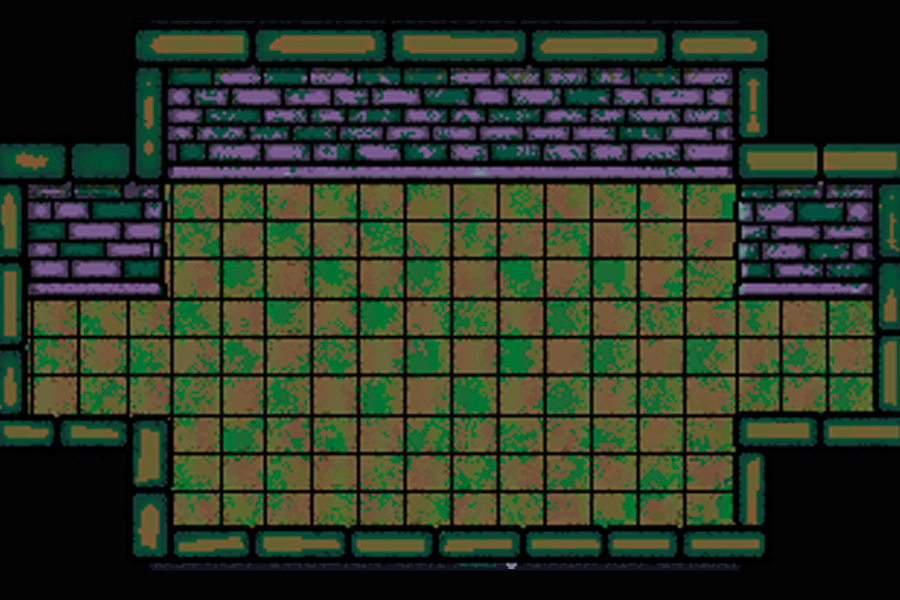
\includegraphics[width=.6\linewidth]{arena_1.png}
                \caption{Segunda arena do jogo}
                \label{fig:arena_1}
            \end{figure}

    \section{Objetos no jogo}
        O único objeto interajível no jogo e que não se move é a porta, que aparece caso não tenha nenhum inimigo na tela e ao ser colidida com o player, leva ele para outra fase.
        
        \begin{figure}[H]
            \centering
            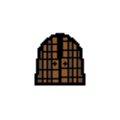
\includegraphics[width=.6\linewidth]{porta.png}
            \caption{Porta para avançar de nível}
            \label{fig:arena}
        \end{figure}

    \section{Personagens do jogo}
        Os personagens do game são os seguintes
        \begin{itemize}
            \item Cavemia
                Se trata do player. É o personagem principal, e ele que será controlado.

                Suas mecânicas incluem:
                \begin{itemize}
                    \item Movimentação
                    \item Colisão com inimigos
                    \item Colisão com porta
                    \item Atirar
                \end{itemize}
                \begin{figure}[H]
                    \centering
                    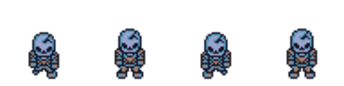
\includegraphics[width=.6\linewidth]{cavemia_frente.png}
                    \caption{Sprite do player}
                    \label{fig:player}
                \end{figure}

            \item Pingoso
                Se trata do primeiro inimigo, tem mais vida mas menos velocidade de movimento.
                
                Suas mecânicas como inimigo incluem:
                \begin{itemize}
                    \item Seguir o player
                    \item Dar dano ao player
                    \item Receber dano do player
                \end{itemize}
                \begin{figure}[H]
                    \centering
                    
\includegraphics[width=.47\linewidth]{pingoso_frente.png}
                    \caption{Sprite do Pingoso}
                    \label{fig:pingoso}
                \end{figure}
            
            \item Fantasgua
                Segundo inimigo, tem menos vida e mais velocidade de movimento.
                
                Por também ser um inimigo, suas mecânicas repetem a do pingoso:
                \begin{itemize}
                    \item Seguir o player
                    \item Dar dano ao player
                    \item Receber dano do player
                \end{itemize}
                \begin{figure}[H]
                    \centering
                    
\includegraphics[width=.6\linewidth]{fantasgua.png}
                    \caption{Sprite do Fantasgua}
                    \label{fig:fantasgua}    
                \end{figure}    
        \end{itemize}

    \section{Objetivo Principal}
        O objetivo principal do jogo é ultrapassar todos os níveis e conseguir sair de sua tumba.
    
    \section{Geração de inimigos}
    A geração de inimigos foi implementada da seguinte forma:
    \subsection{Quantidade de inimigos}
	Foi definido uma função que retorna a quantidade de inimigos para o nível em que o personagem se encontra, sendo da seguinte forma:
	\begin{itemize}
	\item Nivel 1 = Nenhum inimigo
	\item Niveis 2 e 3 = 1 Inimigo
	\item Niveis 4 e 5 = 2 Inimigos
	\item Niveis 6 e 7 = 3 Inimigos 
	\item Niveis 8, 9 e 10 = 4 Inimigos
\end{itemize}	    

	\subsection{Seleção aleatória para a geração de inimigos}
	Para decidir quais inimigos serão gerados, fazemos da seguinte forma:
	\begin{lstlisting}
import random

quantidade_pingoso = random.randint(0, maximo_inimigos)
quantidade_fantasgua = maximo_inimigos - quantidade_pingoso
\end{lstlisting}

Eles são adicionados em uma lista que logo após isso será percorrida por inteiro desenhando todos os elementos com suas posições.

	\subsection{Posição de geração de inimigos}
	Como mencionado anteriormente, os inimigos são adicionados em uma lista para que possa ser percorrido e desenhado na tela. A lista é percorrida da seguinte forma:
	\begin{lstlisting}
	for _ in range(qtdd_fantasgua):
        enemy = Fantasgua(random.randint(0, janela.width), janela.height/2)
        enemies.append(enemy)

    for _ in range(qtdd_pingoso):
        enemy = Pingoso(random.randint(0, janela.width), janela.height/2)
        enemies.append(enemy)

	\end{lstlisting}
	
	Fazendo assim com que sejam gerados no meio da tela (no eixo das ordenadas) e aleatoriamente (no eixo das abscissas).


    
    \section{Controles}
        \begin{itemize}
            \item W: Movimenta o player para cima;
            \item S: Movimenta o player para baixo;
            \item A: Movimenta o player para a esquerda;
            \item D: Movimenta o player para a direita;
            \item Space: Dispara um projétil na direção em que o player está virado.
        \end{itemize}
________________
% chapter Front End
% ______________________


% \chapter{Front End}
% description of front end such as start screen, menu screens,..  

% \section{Start Screen}

% \section{Menus}

% \section{End Screen}

% % ______________________
% % chapter Game Details
% % ______________________


\chapter{Tecnologias}
Por ser um trabalho acadêmico, as tecnologias para o desenvolvimento não permitiam uma engine como a Unreal ou Godot. Todas as mecânicas do jogo foram desenvolvidas puramente por python, por meio da plataforma PPlay. Para a construção dos assets foi utilizado o Aseprite.
\section{PPlay}
PPlay é uma plataforma de desenvolvimento escrito em python como uma forma de releitura, abstração e simplificação do uso do PyGame (Um framework de desenvolvimento de jogos para python). O jogo foi feito utilizando paradigmas de Programação Orientada a Objeto para uma melhor visualização do fluxo de informações, simplificação e prevenção de erros.


\section{Hardware}
Por ser um jogo simples e sem nenhuma engine envolvida, o jogo não precisa de nenhum hardware potente para que seja apreciado.

% ______________________
% chapter Game Details
% ______________________




% ______________________
% chapter Game Details
% ______________________




\end{document}
